\section{Datasets}
\label{sec:datasets}
There are many databases, which provide a lot of datasets. One of those is \textit{kaggle}. \textit{kaggle} does not only provide datasets, they also organize competitions in analyzing datasets or improving already invented algorithms. We found a lot of data about to \textit{New York Stock Exchange}. Unfortunately we did not find one single dataset which satisfied all our requirements. There was no data about how often a search term was requested at \textit{Google}. So we had to collect the data ourselves from \textit{Google Trends}. In the following chapters we describe our datasets and why we are using them.

\subsection{Stock data}
We combined data about the \textit{New York Stock Exchange} of two datasets from \textit{kaggle}.
\label{subsec:stockdata}

\subsubsection{NYSE}
\label{subsub:nyse}
\cite{NYSE} collected information about historical prices of the S\&P 500 companies and additional fundamental data in his dataset. Standard and Poor`s 500 (S\&P 500) is a stock index of the 500 biggest US companies listed on the stock exchange.\\
The dataset has 4 files:
\begin{itemize}
	\item \textbf{prices.csv} This file contains the daily stock prices from 2010 until the end of 2016. For newer companies the range is shorter. Unfortunately the prices are sorted by day and not stock and therefore we could not use this data without preprocessing it. Instead, we found a better suiting dataset.
	\item \textbf{prices-split-adjusted.csv} Approximately 140 stock splits occurred during that time. This file has the same data with adjustments for the splits. We do not use this data neither.
	\item \textbf{fundamentals.csv} The file summarizes some metrics from the annual SECC 10K fillings. The metrics are useless for us, too.
	\item \textbf{securities.csv} Additional information for each stock can be found in this file. The most important data is the mapping from the ticker symbol to the full name of the companies. We use this data as an input for collecting data from \textit{Google Trends}.
\end{itemize}

\subsubsection{S\&P500}
\label{subsub:sp500}
The second dataset from \textit{kaggle} has also information about the daily stock prices from the S\&P 500. \cite{SP500} ordered the prices by stock and are therefore much more useful for us. Each entry consists of the date, four prices, the volume and its ticker symbol. The dataset has the prices for the last five years starting at 2012-08-13 until 2017-08-11. For the weekends there are no entries because the stock market is closed and no trading happens. For our task we use the opening and closing price to calculate if the stock went up or down on one day.


\subsection{Google Trends data}
\label{subsec:gtdata}
Google provides a public accessible service called Google Trends. It offers many different kinds of information about all search terms typed into the Google search engine. For example, for a given search term, like "Commerzbank", a graph is being displayed that shows the number of searches for this exact term over the course of time. The figure \ref{fig:gtexample} depicts a sample of this graph. 
\begin{figure}[!ht]
	\caption{Resulting graph of a google trends \cite{googletrends} search for the financial company "Commerzbank", which is tradeable at the stock market. }
	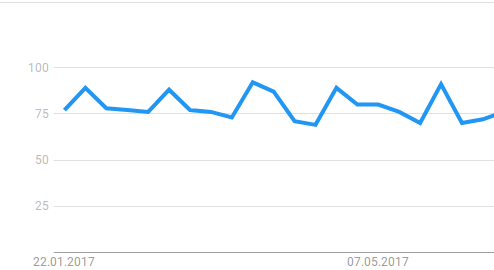
\includegraphics[width=0.95\linewidth]{images/googletrends.png}
	\label{fig:gtexample}
\end{figure}
Additionally, there is other data like the interest grouped by region, related topics and similar search terms available. Especially the similar search terms could be used to traverse all related Google Trends data starting from one single term like a stock course name. Therefore, the simple and automated extraction of Google Trend data is essential for the success of the proposed deep learning model for stock prediction. Unfortunately, there are some problems regarding the automated retrieval of it. This is explained in detail in the following subsection \ref{subsub:hackinggt}.

\subsubsection{Hacking Google Trends}
\label{subsub:hackinggt}
The amount of available data from Google Trends is massive. Unfortunately, unlike many other services of Google, it does not provide a public API for retrieving the trend data. Due to the needed quantity of data, manual extraction is not a practicable option. Therefore, an initial analysis of the sent requests from the web browser was executed. 
\\
The Google Trends website sends an explore-request to collect a JSON-file containing several tokens and further information. These tokens are used by the Google Trends servers to validate a request from the requesting machine to a specific service. The multiline-request is used to retrieve the time line data of a search term. The data for related topics and similar search terms can be collected by the same URL, whereas the respective token needs to be put as value into the token-parameter to distinguish between those two types of information. Based on this analysis, a python script is developed that gathers automatically the needed Google Trends data starting from the stock names. If too many requests are send to the server, the HTML error 429 may occur. This is being take care of by simply waiting a short period of time between the requests. 
\\
However, even the working python script was limited in a way that the Google Trend server only allows a limited number of requests. If that upper bound is reached, the server blocks the requests and redirects to another web address. On this website the user needs to prove that he is not a robot by clicking the parts of a picture that contain a certain object. Although the use of selenium, a framework to automate software tests for web applications, could serve as a possible workaround of this problem, it would imply a huge overhead with uncertain results. Therefore, this option was not further investigated. 
\\
The implemented python script for the automated Google Trend data retrieval, as well as the other related work of this paper, is published in the github repository of \cite{githubrepo}. 

\subsection{Merged dataset}
\label{subsec:merged}
From the three previously described datasets we used only two directly. The NYSE dataset (see \ref{subsub:nyse}) was only used to collect data from \textit{Google Trends} (see \ref{subsec:gtdata}). We combine the data of 14 search terms with the data from S\&P500 (see \ref{subsub:sp500}). We integrated the label in our dataset. The label is calculated from the opening and closing price.
\begin{equation}
y = sign(p_{close} - p_{open})
\end{equation}
The label can be found in the first column so that we can easily extract it in our algorithm. We separate our data in two classes. A label of $1$ means that the stock went up on this day. The other class is labeled with $-1$ and says that the price went down. If the value did not change during the day the label will be $0$. We interpret it the same as the label $-1$ because only up going prices are good if you invested in this stock.\\
The second column contains the opening price we already used to calculate the label. We did not include the closing value because it is the same as the opening price of the following day and could be computed. We include one price so that out network can use it to compare the trend of the stock price with the trends of the search terms. The value may be used to not only predict if the stock goes up or down, but to predict the exact next value.\\
The columns 3 to 16 contain the values of the search terms. It is important that there are only a few values of zeros. One problem is to find good search terms which are really correlated to the trend of the stock price. It is easily possible to replace them and test the network with other search terms. This may improve the prediction. We always include the search terms for the ticker symbol and the company name. The remaining twelve search terms depend on them.\\
Unfortunately it was not possible to collect data from \textit{Google Trends} for all search terms for the last five years. Therefore, we had to discard some of the stock prices and start including them in our dataset as soon as there are enough search terms with a different value than $0$. That is why the trends are starting at a different date.\\
For simplicity we split our dataset into two categories.
\begin{enumerate}
	\item Training and Validation: This dataset contains $209$ entries and can be found in \mbox{\textit{stockprediction/datasets/myDataset}}.
	\item Test: This dataset is used only for testing and never during training. It is located at \mbox{\textit{stockprediction/datasets/testData}} and has $16$ entries which is about $7.66\%$ of the training and validation category.
\end{enumerate}
In the following chapter we describe how and why we preprocess our dataset.
